% Preamble voor de Drainworks-handleiding PDF.
% Wordt door pandoc verbatim ingevoegd via `--include-in-header=preamble.tex`
% (dus GEEN Markdown-verwerking, anders escapet pandoc de [..]-opties).

\usepackage{graphicx}

% Strak schreefloos lettertype (Fira Sans + Fira Mono) i.p.v. het standaard
% Latin Modern. De fonts komen uit tectonic's eigen bundel (laden op
% bestandsnaam). Renderer=OpenType is nodig omdat tectonic's HarfBuzz-renderer
% op deze OTF's crasht.
\setmainfont{FiraSans-Regular.otf}[Renderer=OpenType, BoldFont=FiraSans-Bold.otf, ItalicFont=FiraSans-Italic.otf, BoldItalicFont=FiraSans-BoldItalic.otf]
\setmonofont{FiraMono-Regular.otf}[Renderer=OpenType, BoldFont=FiraMono-Bold.otf]

% Symbolen die de bodyfont mist (✓ ⚠ ✕ ↶ ↷) vervangen door equivalenten uit
% pifont/amssymb/FontAwesome, zodat ze niet leeg in de PDF verschijnen. De
% FontAwesome-driehoek laadt de font direct (het fontawesome5-pakket dwingt de
% crashende HarfBuzz-renderer af).
\usepackage{amssymb}
\usepackage{pifont}
\newfontface\fawarnfont[Renderer=OpenType]{FontAwesome5Free-Solid-900.otf}
\usepackage{newunicodechar}
\newunicodechar{✓}{\ding{51}}
\newunicodechar{✕}{\ding{55}}
\newunicodechar{⚠}{{\fawarnfont\symbol{"F071}}}
\newunicodechar{↶}{\ensuremath{\curvearrowleft}}
\newunicodechar{↷}{\ensuremath{\curvearrowright}}

% Optionele omslagafbeelding op de titelpagina: plaats screenshots/00-omslag.png
% en haal de onderstaande regel uit commentaar.
% \titlegraphic{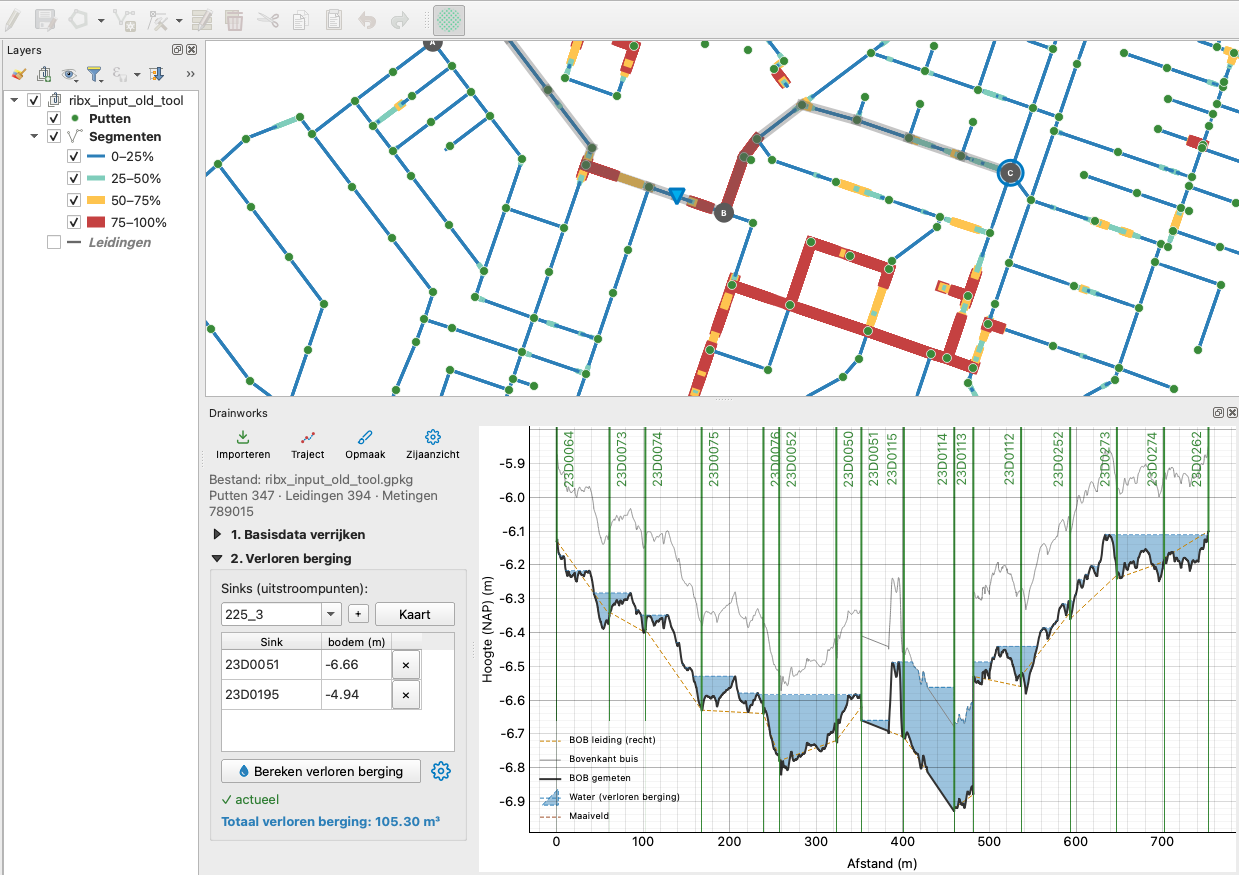
\includegraphics[width=0.6\textwidth]{screenshots/00-omslag.png}}
